\documentclass[10pt, a4paper]{exam}
%\printanswers			    % Comment this line to hide the answers 
\usepackage[utf8]{inputenc}
\usepackage[T1]{fontenc}
\usepackage[ngerman]{babel}
\usepackage{enumitem,amsmath,amsthm,amsfonts,amssymb}
\usepackage{color,graphicx,overpic}
\usepackage{hyperref}
\usepackage{pgfplots}
\usepackage{bussproofs}
\usepackage[many]{tcolorbox}

% Don't print section numbers
\setcounter{secnumdepth}{0}
\qformat{\textbf{Aufgabe \thequestion}\dotfill \thepoints}

\pdfinfo{
  /Title (Logik und Logikprogrammierung - Übung)
  /Creator (TeX)
  /Producer (pdfTeX 1.40.0)
  /Subject ()
}
\title{Logik und Logikprogrammierung - Übung}
\author{}
\date{}

\newtcolorbox{myboxii}[1][]{
  breakable,
  freelance,
  title=#1,
  colback=white,
  colbacktitle=white,
  coltitle=black,
  fonttitle=\bfseries,
  bottomrule=0pt,
  boxrule=0pt,
  colframe=white,
  overlay unbroken and first={
  \draw[red!75!black,line width=3pt]
    ([xshift=5pt]frame.north west) -- 
    (frame.north west) -- 
    (frame.south west);
  \draw[red!75!black,line width=3pt]
    ([xshift=-5pt]frame.north east) -- 
    (frame.north east) -- 
    (frame.south east);
  },
  overlay unbroken app={
  \draw[red!75!black,line width=3pt,line cap=rect]
    (frame.south west) -- 
    ([xshift=5pt]frame.south west);
  \draw[red!75!black,line width=3pt,line cap=rect]
    (frame.south east) -- 
    ([xshift=-5pt]frame.south east);
  },
  overlay middle and last={
  \draw[red!75!black,line width=3pt]
    (frame.north west) -- 
    (frame.south west);
  \draw[red!75!black,line width=3pt]
    (frame.north east) -- 
    (frame.south east);
  },
  overlay last app={
  \draw[red!75!black,line width=3pt,line cap=rect]
    (frame.south west) --
    ([xshift=5pt]frame.south west);
  \draw[red!75!black,line width=3pt,line cap=rect]
    (frame.south east) --
    ([xshift=-5pt]frame.south east);
  },
}

\begin{document}
\begin{myboxii}[Disclaimer]
    Die Übungen die hier gezeigt werden stammen aus der Vorlesung \textit{Logik und Logikprogrammierung}! Für die Richtigkeit der Lösungen wird keine Gewähr gegeben.
\end{myboxii}

\begin{questions}
    \question Emil hat seine Freunde Anne, Bernd, Christiane und Dirk auf eine Party eingeladen. Leider gibt es dabei einige Komplikationen.
    \begin{enumerate}
        \item Anne ist in Bernd verliebt und kommt nur mit, wenn Bernd auch kommt.
        \item Bernd ist jedoch in Christiane verliebt und kommt nur, wenn Christiane auch kommt.
        \item Zudem ist auch Dirk in Christiane verliebt und, falls Christiane kommt, kommt Dirk auch.
        \item Wenn Dirk mitkommt, wird er auf jeden Fall Anne oder Bernd mitbringen.
        \item Christiane ist die Situation peinlich und kommt, falls sowohl Bernd als auch Dirk mitkommen, nicht mit.
    \end{enumerate}

    \begin{parts}
        \part Formalisieren Sie die gegebenen Sachverhalte durch aussagenlogische Formeln.Hinweis: Die Motivationsgründe der einzelnen Personen können dabei vernachlässigt werden. Verwenden Sie die atomaren Formeln A für ,,Anne kommt mit'', B für ,,Bernd kommt mit'', C für ,,Christiane kommt mit'' und D für ,,Dirk kommt mit''.
        \begin{solution}
            \begin{enumerate}
                \item $A\rightarrow B$
                \item $B\rightarrow C$
                \item $C\rightarrow D$
                \item $D\rightarrow (A\vee B)$
                \item $(B\wedge D) \rightarrow \lnot C$
            \end{enumerate}
        \end{solution}

        \part Argumentieren Sie, dass keiner der vier Freunde Emils zur Party mitkommt.
        \begin{solution}

            Ziel: $\lnot A \wedge \lnot B \wedge \lnot C \wedge \lnot D$                                              \\
            Es gilt: $B\rightarrow D$, da $B\rightarrow C$ und $C\rightarrow D$                                       \\
            Es gilt: $D\rightarrow B$, da $D\rightarrow (A\vee B)$ und $A\rightarrow B$                               \\
            Es gilt: $B\leftrightarrow D$, da $B\rightarrow D$ und $D\rightarrow B$                                   \\
            Es gilt: $C\rightarrow B$, da $C\rightarrow D$ und $D\rightarrow B$                                       \\
            Es gilt: $B\leftrightarrow C$, da $B\rightarrow C$ und $C\rightarrow B$                                   \\
            Es gilt äquivalenz: $(\lnot B\wedge \lnot C\wedge \lnot D)\vee(B\wedge C\wedge D)$                        \\
            Angenommen $B\wedge C\wedge D$, dann $B\wedge D\Rightarrow \lnot C$, also $\lnot C$ und $C$ !Widerspruch! \\
            Es gilt: $\lnot A$, da $A\rightarrow B$ und $\lnot B$                                                     \\
            Es gilt $\lnot A\wedge \lnot B\wedge \lnot C\wedge \lnot D$
        \end{solution}
    \end{parts}

    \question Sei $P=\{p_1,...,p_k\}$ eine endliche, nicht-leere Menge atomarer Formeln. Wir können die Menge $AL(P)$ der aussagenlogischen Formeln über den atomaren Formeln aus $P$ als eine formale Sprache über dem Alphabet $\sum=\{\bot,\wedge,\vee,\rightarrow,\lnot,(,)\} \vee P$ auffassen.

    \begin{parts}
        \part Zeigen Sie, dass $AL(P)$ nicht regulär ist.
        \begin{solution}
            Mit Satz von Myhill-Nerode: Betrachte Wörter $v_n=[(P_n)]^n P_n$. Für $m\not = n$ sind $v_m, v_n$ in verschiedenen MN-Äquivalenzklassen:
            $v_m[I]^m \in AL(P)$ und $v_n[I]^m \not\in AL(P)$ \\
            Also gibt es unendlich viele MN-Äquivalenzklassen und $AL(P)$ ist nicht regulär
        \end{solution}

        \part Zeigen Sie, dass $AL(P)$ jedoch kontextfrei ist, indem Sie eine kontextfreie Grammatik angeben, die $AL(P)$ erzeugt.
        \begin{solution}

            $G=(V,\sum,P,S)$ \\
            $S\rightarrow \bot |p_1|...|p_k|\lnot S| (S\wedge S) | (S\vee S) | (S\rightarrow S)$
        \end{solution}

    \end{parts}

    \question Zeigen Sie per vollständiger Induktion über den Formelaufbau, dass in jeder Formel die Anzahl der öffnenden Klammern gleich der Anzahl der schließenden Klammern ist, d.h. zeigen Sie, dass für alle endlichen Mengen atomarer Formeln $P=\{p_1,...,p_k\}$ und alle $\phi\in AL(P)$, dass $|\phi|_(=|\phi|_)$ gilt.

    \begin{solution}

        Induktion über Formelaufbau.                                                                             \\
        I.A.: $E=\bot: |\bot|_) = 0 = |\bot|_($, $E=p_i: |p_i|_) = 0 = |p_i|_($                                  \\
        I.V.: für $E,\Phi \in AL(P)$ gilt $|E|_( = |E|_)$,$|\Phi|_(=|\Phi|_)$                                    \\
        I.S.: $\lnot E: |\lnot E|_( = |\lnot |_( +|E|_( = |\lnot|_(+|E|_) = |E|_)= |\lnot|_)+|E|_)= |\lnot E|_)$ \\
        $\quad\quad (E\wedge \Phi): |(E\wedge\Phi)|_(= |(|_( + |E|_( + |\wedge| + |\Phi|_( + |)|_( = 1 + |E|_( + |\Phi|_( +0 = 1+|E|_)+0+|\Phi|_) = |(|_) + |E|_) + |\wedge| + |\Phi|_) + |)|_) = |(E\wedge\Phi)_)$
        \\$(E\vee\Phi), (E\rightarrow\Phi)$ analog
    \end{solution}

    \question Seien $\phi, \psi$ aussagenlogische Formeln. Wir sagen, dass $\psi$ eine Teilformel von $\phi$ ist wenn $\phi$ (als syntaktisches Wort) ein Infix von $\psi$ ist. Zum Beispiel ist $p_1$ eine Teilformel von $\lnot (p_2\wedge p_1)$, nicht aber $\lnot($, da dies keine aussagenlogische Formel ist. Sei $TF(\phi)$ die Anzahl der Teilformeln von $\phi$. Zeigen Sie per vollständiger Induktion über den Formelaufbau, dass für jede aussagenlogische Formel $\phi$ die Anzahl der Teilformeln von $\phi$ kleiner gleich der Länge von $\phi$ ist, also $TF(\phi) \leq |\phi|$.

    \begin{solution}

        I.A.: $E =\bot: TF(\bot) = 1 = |E|, \quad E=p_i: TF(p_i) = 1 = |E|$

        I.V.: gelte für Formel $E, \Psi$, d.h. $TF(E) \leq |E|$ und $TF(\Psi) \leq |\Psi|$

        I.S.:
        \begin{itemize}
            \item $\lnot E:TF(\lnot E)\leq 1 + TF(E) \leq 1+|E| = |\lnot E|$
            \item $(E\wedge \Psi): TF(E\wedge\Psi)=1+TF(E)+TF(\Psi) \leq 1+|E|+|\Psi| \leq 3+|E|+|\Psi|=|(E\wedge\Psi)|$
            \item $(E\vee\Psi), (E\rightarrow\Psi)$ analog
        \end{itemize}

        Also folgt aus der vollständigen Induktion
    \end{solution}

    \question Vervollständigen Sie die folgende Deduktion um die angewendeten Regeln, gestrichenen Hypothesen und fehlenden Formeln. Markieren Sie zudem für alle gestrichenen Hypothesen, durch welche Regelanwendung diese gestrichen wurden.
    \begin{prooftree}
        \AxiomC{$\phi\vee\psi$}
        \AxiomC{$\lnot \phi\wedge\lnot\psi$}
        \RightLabel{\scriptsize ($\wedge E_1$)}
        \UnaryInfC{?}
        \AxiomC{$\phi$}
        \RightLabel{\scriptsize ($\lnot E$)}
        \BinaryInfC{?}
        \RightLabel{\scriptsize ($\lnot I$)}
        \UnaryInfC{$\lnot(\lnot \phi\wedge\lnot\psi)$}
        \AxiomC{$\lnot\phi\wedge\lnot\psi$}
        \RightLabel{\scriptsize ($\wedge E_2$)}
        \UnaryInfC{?}
        \AxiomC{$\psi$}
        \RightLabel{\scriptsize ($\lnot E$)}
        \BinaryInfC{?}
        \RightLabel{\scriptsize ($\lnot I$)}
        \UnaryInfC{$\lnot(\lnot\phi\wedge\lnot\psi$)}
        \TrinaryInfC{$\lnot(\lnot\phi\wedge\lnot\psi)$}
        \UnaryInfC{$\lnot B$}
    \end{prooftree}

    \begin{solution}
        \begin{prooftree}
            \AxiomC{$\phi\vee\psi$}
            \AxiomC{$[\lnot \phi\wedge\lnot\psi]^2$}
            \RightLabel{\scriptsize ($\wedge E_1$)}
            \UnaryInfC{$\lnot\phi$}
            \AxiomC{$[\phi]^1$}
            \RightLabel{\scriptsize ($\lnot E$)}
            \BinaryInfC{$\bot$}
            \RightLabel{\scriptsize ($\lnot I (2)$)}
            \UnaryInfC{$\lnot(\lnot \phi\wedge\lnot\psi)$}
            \AxiomC{$[\lnot\phi\wedge\lnot\psi]^3$}
            \RightLabel{\scriptsize ($\wedge E_2$)}
            \UnaryInfC{$\lnot\psi$}
            \AxiomC{$[\psi]^1$}
            \RightLabel{\scriptsize ($\lnot E$)}
            \BinaryInfC{$\bot$}
            \RightLabel{\scriptsize ($\lnot I (3)$)}
            \UnaryInfC{$\lnot(\lnot\phi\wedge\lnot\psi$)}
            \RightLabel{\scriptsize ($\vee E (1)$)}
            \TrinaryInfC{$\lnot(\lnot\phi\wedge\lnot\psi)$}
            \UnaryInfC{$\lnot B$}
        \end{prooftree}
    \end{solution}

    \question In Aufgabe 1 haben wir einen Sachverhalt durch folgende Formeln formalisiert:
    $$A\rightarrow B, B\rightarrow C, C\rightarrow D, D\rightarrow(A\vee B), (B\wedge D)\rightarrow\lnot C$$
    Konstruieren Sie eine formale Deduktion von $\lnot B$, die nur diese Formeln als Hypothesen nutzt (alle anderen Hypothesen sind gestrichen).

    \begin{solution}

        \textbf{Version 1:}
        \begin{prooftree}
            \AxiomC{$(B\wedge D)\rightarrow \lnot C$}
            \AxiomC{$B\rightarrow C$}
            \AxiomC{$C\rightarrow D$}
            \BinaryInfC{$B\rightarrow D$}
            \AxiomC{$D\rightarrow (A\vee B)$}
            \AxiomC{$A\rightarrow B$}
            \BinaryInfC{$D\rightarrow B$}
            \BinaryInfC{$B\leftrightarrow D$}
            \AxiomC{$C\rightarrow D$}
            \AxiomC{$D\rightarrow B$}
            \BinaryInfC{$C\rightarrow B$}
            \AxiomC{$B\rightarrow C$}
            \BinaryInfC{$B\leftrightarrow C$}
            \BinaryInfC{$(\lnot B\wedge\lnot C\wedge\lnot D)\vee(B\wedge C\wedge D)$}
            \BinaryInfC{$\lnot B \wedge \lnot C \wedge \lnot D$}
            \UnaryInfC{$\lnot B$}
        \end{prooftree}

        \textbf{Version 2:}
        \begin{prooftree}
            \AxiomC{$[B]^1$}
            \AxiomC{$B\rightarrow C$}
            \RightLabel{\scriptsize ($\rightarrow E$)}
            \BinaryInfC{$C$}
            \AxiomC{$[B]^1$}
            \AxiomC{$[B]^1$}
            \AxiomC{$B\rightarrow C$}
            \BinaryInfC{$C$}
            \AxiomC{$C\rightarrow D$}
            \RightLabel{\scriptsize ($\rightarrow I$)}
            \BinaryInfC{$D$}
            \BinaryInfC{$(B\wedge D)$}
            \AxiomC{$(B\wedge D)\rightarrow \lnot C$}
            \RightLabel{\scriptsize ($\rightarrow E$)}
            \BinaryInfC{$\lnot C$}
            \BinaryInfC{$\bot$}
            \RightLabel{\scriptsize ($\lnot I (1)$)}
            \UnaryInfC{$\lnot B$}
        \end{prooftree}
    \end{solution}

    \question Wir wollen in dieser Aufgabe zeigen, dass in der Aussagenlogik sowohl Konjunktion als auch Disjunktion assoziativ sind. Seien dazu $p_1, p_2, p_3$ aussagenlogische Formeln.

    \begin{parts}
        \part Zeigen Sie, dass $\{p_1\wedge(p_2\wedge p_3)\}\vdash(p_1\wedge p_2)\wedge p_3$ gilt.
        \begin{solution}
            \begin{prooftree}
                \AxiomC{$p_1\wedge(p_2\wedge p_3)$}
                \RightLabel{\scriptsize ($\wedge E_1$)}
                \UnaryInfC{$p_1$}
                \AxiomC{$p_1\wedge(p_2\wedge p_3)$}
                \RightLabel{\scriptsize ($\wedge E_2$)}
                \UnaryInfC{$(p_2\wedge p_3)$}
                \RightLabel{\scriptsize ($\wedge E_1$)}
                \UnaryInfC{$p_2$}
                \RightLabel{\scriptsize ($\wedge I$)}
                \BinaryInfC{$(p_1\wedge p_2)$}
                \AxiomC{$p_1\wedge(p_2\wedge p_3)$}
                \RightLabel{\scriptsize ($\wedge E_2$)}
                \UnaryInfC{$(p_2\wedge p_3)$}
                \RightLabel{\scriptsize ($\wedge E_2$)}
                \UnaryInfC{$p_3$}
                \RightLabel{\scriptsize ($\wedge I$)}
                \BinaryInfC{$(p_1 \wedge p_2)\wedge p_3$}

            \end{prooftree}

            Also gilt ${p_1\wedge(p_2\wedge p_3)}\vdash (p_1\wedge p_2)\wedge p_3$
        \end{solution}


        \part Zeigen Sie, dass $\{p1\vee (p_2\vee p_3)\}\vdash(p_1\vee p_2)\vee p_3$ gilt, indem Sie die folgende Deduktion vervollständigen.
        \begin{solution}
            \begin{prooftree}
                \AxiomC{$p_1\vee(p_2\vee p_3)$}
                \AxiomC{$[p_1]^1$}
                \RightLabel{\scriptsize ($\vee I_1$)}
                \UnaryInfC{$(p_1\vee p_2)$}
                \RightLabel{\scriptsize ($\vee I_2$)}
                \UnaryInfC{$(p_1\vee p_2)\vee p_3$}
                \AxiomC{$[(p_2\vee p_3)]^1$}
                \AxiomC{$[p_2]^2$}
                \RightLabel{\scriptsize ($\vee I_2$)}
                \UnaryInfC{$(p_1\vee p_2$)}
                \RightLabel{\scriptsize ($\vee I_1$)}
                \UnaryInfC{$(p_1\vee p_2)\vee p_3$}
                \AxiomC{$[p_2]^2$}
                \RightLabel{\scriptsize ($\vee I_2$)}
                \UnaryInfC{$(p_1\vee p_2)\vee p_3$}
                \RightLabel{\scriptsize ($\vee E (2)$)}
                \TrinaryInfC{$(p_1\vee p_2)\vee p_3$}
                \RightLabel{\scriptsize ($\vee E (1)$)}
                \TrinaryInfC{$(p_1\vee p_2)\vee p_3$}
            \end{prooftree}

            Also gilt ${p_1\vee(p_2\vee p_3)}\vdash (p_1\vee p_2)\vee p_3$
        \end{solution}

    \end{parts}

    \question Werten Sie die folgenden Formeln für die jeweils angegebene Belegung aus.

    \begin{parts}
        \part $p_1\rightarrow(p_2\wedge p_3)$ für die $K_3$-Belegung mit $B(p_1)=\frac{1}{2}, B(p_2)=1$ und $B(p_3)=0$
        \begin{solution}
            $B(p_1\rightarrow (p_2\wedge p_3)) = max (...)$
        \end{solution}

        \part $(p_1\vee p_2)\rightarrow(p_2\wedge p_3)$ für die $F$-Belegung mit $B(p_1)=0.3, B(p_2)=0.7$ und $B(p_3)=1$
        \begin{solution}
            $B((p_1\vee p_2)\rightarrow(p_2\wedge p_3) = max(B(p_2\wedge p_3), 1-B(p_1\vee p_2)) = max(min(B(p_2),B(p_3)), 1-max(B(p_1),B(p_2))) = max(min(0.7,1),1-max(0.5,0.7)) = 0.7$
        \end{solution}

        \part $\lnot(p_1\rightarrow(p_2\wedge p_3))$ für die $B_R$-Belegung mit $B(p_1)=\mathbb{R}, B(p_2)=[1,\pi]$ und $B(p_3)=[3,42]$
        \begin{solution}
            $B(\lnot(p_1\rightarrow(p_2\wedge p_3)))=\mathbb{R}\backslash B(p_1\rightarrow (p_2\wedge p_3)) = \mathbb{R}\backslash(B(p_2\wedge p_3)\cup(\mathbb{R}\backslash B(p_1))) = \mathbb{R}\backslash[(B(p_2)\cap B(p_3))\cup(\mathbb{R}\backslash B(p_1))]= \mathbb{R}\backslash[[1,\pi]\cap [3,42]\cup\mathbb{R}\backslash\mathbb{R}]=\mathbb{R}\backslash[3,\pi]$
        \end{solution}

        \part $p_1\rightarrow(p_2\wedge p_3)$ für die $H_{mathbb{R}}$-Belegung mit $B(p_1)=\mathbb{R}_{>0}, B(p_2)=(-10,5)$ und $B(p_3)=(-20,-3)$
        \begin{solution}
            $B(p_1\rightarrow (p_2\wedge p_3))= Inneres(B(p_2\wedge p_3), \mathbb{R}\backslash B(p_1))= Inneres(B(p_1)\cap B(p_2), \mathbb{R}\backslash B(p_1))= Inneres(\mathbb{R}_{\leq 0}) = \mathbb{R}_{< 0}$
        \end{solution}
    \end{parts}

    \question Bearbeiten Sie die folgenden Teilaufgaben
    \begin{parts}
        \part Entscheiden Sie welche der folgenden Paare $\Gamma\Vdash_W \varphi$ erfüllen. Beweisen Sie Ihre Behauptung zum Beispiel durch Angabe einer Wahrheitstabelle.
        \begin{subparts}
            \subpart $\Gamma=\{p_1\rightarrow p_1\}, \varphi=p_1, W\in\{B,K_3\}$

            \begin{solution}

                \begin{tabular}{c|c|c}
                    $p_1$ & $p_1\rightarrow p_1$ & $p_1\rightarrow p_1 \Vdash p_1$ \\\hline
                    w     & w                    & w                               \\
                    $0.5$ & w                    & w                               \\
                    f     & w                    & w                               \\
                \end{tabular}
            \end{solution}

            \subpart $\Gamma=\{p_1\rightarrow p_2, p_1\}, \varphi=p_2, W\in\{B,K_3\}$
            \begin{solution}

                \begin{tabular}{c | c | c | c}
                    $p_1$ & $p_2$ & $p_1\rightarrow p_2$ & $p_1\rightarrow p_2\Vdash p_2$ \\\hline
                    w     & w     & w                    & w                              \\
                    w     & $0.5$ & w                    & w                              \\
                    w     & f     & f                    & w                              \\
                    $0.5$ & w     & w                    & w                              \\
                    $0.5$ & $0.5$ & w                    & w                              \\
                    $0.5$ & f     & f                    & w                              \\
                    f     & w     & w                    & f                              \\
                    f     & $0.5$ & w                    & f                              \\
                    f     & f     & w                    & f                              \\
                \end{tabular}
            \end{solution}

            \subpart $\Gamma=\{p_3\vee(p_1\wedge p_2)\}, \varphi=(p_3\vee p_1)\wedge(p_3\vee p_2), W\in\{B\}$
            \begin{solution}

                \begin{tabular}{c | c | c | c | c | c | c | c | c}
                    $p_1$ & $p_2$ & $p_3$ & $p_1\wedge p_2$ & $p_3\vee(p_1\wedge p_2)$ & $p_3\vee p_1$ & $p_3\vee p_2$ & $(p_3\vee p_1)\wedge(p_3\vee p_2)$ & $p_3\vee(p_1\wedge p_2) \Vdash (p_3\vee p_1)\wedge(p_3\vee p_2)$ \\\hline
                    w     & w     & w     & w               & w                        & w             & w             & w                                  & $\leftrightarrow$                                                \\
                    w     & w     & f     & w               & w                        & w             & w             & w                                  & $\leftrightarrow$                                                \\
                    w     & f     & w     & f               & w                        & w             & w             & w                                  & $\leftrightarrow$                                                \\
                    w     & f     & f     & f               & f                        & w             & f             & f                                  & $\leftrightarrow$                                                \\
                    f     & w     & w     & f               & w                        & w             & w             & w                                  & $\leftrightarrow$                                                \\
                    f     & w     & f     & f               & f                        & f             & w             & f                                  & $\leftrightarrow$                                                \\
                    f     & f     & w     & f               & w                        & w             & w             & w                                  & $\leftrightarrow$                                                \\
                    f     & f     & f     & f               & f                        & f             & f             & f                                  & $\leftrightarrow$                                                \\
                \end{tabular}
            \end{solution}
        \end{subparts}

        \part Entscheiden Sie für $W\in\{B,K_3\}$, welche der folgenden Formeln W-Tautologie sind. Beweisen Sie Ihre Behauptung.
        \begin{subparts}
            \subpart $\lnot(p_1\wedge \lnot p_1)$
            \begin{solution}

                \begin{tabular}{c | c | c | c}
                    $p_1$ & $\lnot p_1$ & $p_1\wedge \lnot p_1$ & $\lnot(p_1\wedge \lnot p_1)$ \\\hline
                    w     & f           & f                     & w                            \\
                    f     & w           & f                     & w
                \end{tabular}

                $\Rightarrow Tautologie$
            \end{solution}

            \subpart $\lnot(p_1\wedge\bot)$
            \begin{solution}

                \begin{tabular}{c | c | c}
                    $p_1$ & $p_1\wedge \bot$ & $\lnot(p_1\wedge \bot)$ \\\hline
                    w     & f                & w                       \\
                    f     & f                & w
                \end{tabular}

                $\Rightarrow Tautologie$
            \end{solution}

            \subpart $(p_1\vee p_2 \vee p_3)\rightarrow(p_1\rightarrow(p_2\rightarrow p_3))$
            \begin{solution}

                \begin{tabular}{c | c | c | c | c | c | c}
                    $p_1$ & $p_2$ & $p_3$ & $A=p_1\vee p_2\vee p_3$ & $p_2\rightarrow p_3$ & $B=p_1\rightarrow(p_2\rightarrow p_3)$ & $A\rightarrow B$ \\\hline
                    w     & w     & w     & w                       & w                    & w                                      & w                \\
                    w     & w     & f     & w                       & f                    & f                                      & w                \\
                    w     & f     & w     & w                       & w                    & w                                      & w                \\
                    w     & f     & f     & w                       & w                    & w                                      & w                \\
                    f     & w     & w     & w                       & w                    & w                                      & w                \\
                    f     & w     & f     & w                       & f                    & w                                      & w                \\
                    f     & f     & w     & w                       & w                    & w                                      & w                \\
                    f     & f     & f     & f                       & w                    & w                                      & w
                \end{tabular}

                $\Rightarrow Tautologie$
            \end{solution}
        \end{subparts}
    \end{parts}

    \question Wir erweitern die Aussagenlogik um den zweistelligen Operator $\bar{\wedge}$ (nicht . . . und . . . ).

    \begin{parts}
        \part Überlegen Sie sich, wie Sie eine Aussage ,,nicht ($\varphi$ und $\psi$ )'' beweisen bzw. in einem Beweis verwenden würden und geben Sie entsprechende Regeln $(\bar{\wedge}I)$ und ($\bar{\wedge}E$) an.
        Hinweis: Orientieren Sie sich für $(\bar{\wedge}E$) an der Regel ($\vee E$) und nutzen Sie, dass $\varphi\bar{\wedge}\psi\equiv\lnot \varphi\vee\lnot\psi$.
        \begin{solution}

            \begin{tabular}{c | c | c}
                $\varphi$ & $\psi$ & $\varphi\bar{\wedge}\psi$ \\\hline
                w         & w      & f                         \\
                w         & f      & w                         \\
                f         & w      & w                         \\
                f         & f      & w
            \end{tabular}

            \begin{prooftree}
                \AxiomC{$\lnot\varphi$}
                \RightLabel{\scriptsize ($\bar{\wedge} I_1$)}
                \UnaryInfC{$\lnot(\varphi \wedge\psi)$}
            \end{prooftree}

            \begin{prooftree}
                \AxiomC{$\lnot\psi$}
                \RightLabel{\scriptsize ($\bar{\wedge} I_2$)}
                \UnaryInfC{$\lnot(\varphi \wedge\psi)$}
            \end{prooftree}

            \begin{prooftree}
                \AxiomC{$\lnot(\varphi \wedge\psi)$}
                \RightLabel{\scriptsize ($\bar{\wedge} E_1$)}
                \UnaryInfC{$\varphi$}
            \end{prooftree}

            \begin{prooftree}
                \AxiomC{$\lnot(\varphi \wedge \psi)$}
                \RightLabel{\scriptsize ($\bar{\wedge} E_2$)}
                \UnaryInfC{$\psi$}
            \end{prooftree}
        \end{solution}

        \part Verwenden Sie die Regel aus Aufgabenteil (a), um zu zeigen, dass $p_1\bar{\wedge}\lnot p_1$ ein Theorem ist.
        \begin{solution}

            \begin{tabular}{c | c | c | c}
                $p_1$ & $\lnot p_1$ & $p_1\wedge \lnot p_1$ & $\lnot(p_1\wedge \lnot p_1)$ \\\hline
                w     & f           & f                     & w                            \\
                f     & w           & f                     & w
            \end{tabular}
        \end{solution}

        \part Beschreiben Sie die Semantik des Operators durch Angabe einer Funktion $\bar{\wedge}_W$ wie auf den Folien 3.9ff für die Wahrheitswertebereiche $W\in\{B,B_R,K_3,F\}$.
        \begin{solution}

            \begin{description}
                \item[Wahrheitswertebereich $B$] $a \bar{\wedge}_W b = \lnot(a\wedge b) = \lnot(max(a,b))$
                \item[Wahrheitswertebereich $B_\mathbb{R}$] $a \bar{\wedge}_W b = \lnot(a\wedge b) = \lnot(a\cup b)$
                \item[Wahrheitswertebereich $K_3$] $a \bar{\wedge}_W b = \lnot(a\wedge b) = \lnot(max(a,b))$
                \item[Wahrheitswertebereich $F$] $a \bar{\wedge}_W b = \lnot(a\wedge b) = \lnot(max(a,b))$
            \end{description}
        \end{solution}

        \part Überprüfen Sie, ob die Formel $(p_1\rightarrow p_2)\bar{\wedge}\lnot p_1$ eine W-Tautologie ist für $W\in\{B,K_3,B_R\}$.
        \begin{solution}

            \begin{tabular}{c | c | c | c | c}
                $p_1$ & $p_2$ & $p_1\rightarrow p_2$ & $\lnot p_1$ & $(p_1\rightarrow p_2)\bar{\wedge}\lnot p_1$ \\\hline
                w     & w     & w                    & f           & w                                           \\
                w     & $0.5$ & w                    & f           & w                                           \\
                w     & f     & f                    & f           & w                                           \\
                $0.5$ & w     & w                    & $0.5$       & f                                           \\
                $0.5$ & $0.5$ & w                    & $0.5$       & f                                           \\
                $0.5$ & f     & f                    & $0.5$       & w                                           \\
                f     & w     & w                    & w           & f                                           \\
                f     & $0.5$ & w                    & w           & f                                           \\
                f     & f     & w                    & w           & f
            \end{tabular}
            $\not\Rightarrow Tautologie$
        \end{solution}

        \part Angenommen wir erweitern die Regeln des natürlichen Schließens um $(\bar{\wedge}I)$ und $(\bar{\wedge}E)$. Geben Sie zum Beweis des Korrektheitslemmas für das natürliche Schließen und den Wahrheitswertebereich $B$ den Induktionsschritt für diese Regeln an.
        \begin{solution}

        \end{solution}

        \part Zeigen Sie per vollständiger Induktion über den Formelaufbau, dass es zu jeder aussagenlogischen Formel $\varphi$ eine Formel $\psi$ gibt, die nur $\bar{\wedge}$ als Operator enthält und äquivalent zu $\varphi$ ist, $\varphi\equiv\psi$.
        \begin{solution}

        \end{solution}
    \end{parts}

    \question Zeigen Sie (kurz) die folgenden Aussagen.
    \begin{parts}
        \part Die Formelmenge $\{\varphi\}$ ist erfüllbar genau dann, wenn $\lnot\varphi$ kein Theorem ist.
        \begin{solution}
            $\varnothing\not\vdash\lnot\varphi \Vdash \{\varphi\}$
        \end{solution}

        \part Wenn $\varphi$ eine F-Tautologie ist, dann ist $\bot$ eine Teilformel von $\varphi$.
        \begin{solution}
            $\Gamma\Vdash_F \rightarrow \varphi\rightarrow\bot$
        \end{solution}

        \part Das natürliche Schließen ist auch ohne die Regel $(\bot)$ vollständig.
        \begin{solution}

        \end{solution}

        \part Für jede aussagenlogische Formel $\varphi$ gibt es unendlich viele, paarweise verschiedene, äquivalente Formeln.
        \begin{solution}

            Idee: Kombination der Menge mit beliebige u.u. unendlich vielen Formeln $\lnot\bot$

            unendlich viele, da $\wedge(\lnot\bot)$ unendlich oft zusammenhängen kann

            paarweise verschieden, da $\phi(\wedge(\lnot\bot))^n \not=\phi(\wedge(\lnot\bot))^m$

            äquivalent: $\wedge(\lnot\bot)$ ändert den Wert einer Formel nicht
        \end{solution}
    \end{parts}

    \question Sei $T=(V,E,w)$ ein endlich verzweigter Baum mit Wurzelwund unendlich vielen Knoten.
    \begin{parts}
        \part Beschreiben Sie mit einer Formelmenge $\Gamma_T$, dass in $T$ ein unendlicher Pfad von der Wurzel aus existiert. Verwenden Sie atomare Formeln $\{p_v|v\in V\}$, wobei $p_v$ die intendierte Bedeutung „der Knoten $v$ liegt auf einem unendlichen Pfad von der Wurzel aus“ hat.\\
        Hinweis: D.h. $\Gamma_T$ ist eine Formelmenge, sodass die unendlichen Pfade von $w$ aus in $T$ genau die sind, die die Form $\{v|B(p_v)=1\}$ haben für eine passende Belegung $B$ mit $B(\gamma)=1$ für alle $\gamma\in\Gamma_T$.
        \begin{solution}

        \end{solution}

        \part Verwenden Sie den Kompaktheitssatz der Aussagenlogik um zu beweisen, dass $T$ einen unendlichen Pfad von der Wurzel aus besitzt.\\
        Hinweis: Zeigen Sie zunächst, dass $T$ beliebig lange Pfade von der Wurzel aus besitzt.
        \begin{solution}

        \end{solution}
    \end{parts}

    \question Bearbeiten Sie die folgenden Teilaufgaben!
    \begin{parts}
        \part Überprüfen Sie mittels Makierungsalgorithmus, ob die unten angegebene Folgerung gilt.
        $$p_1\wedge (p_2\vee \lnot p_3\vee \lnot p_5)\wedge (\lnot p_1\vee p_3)\wedge (\lnot p_3\vee p_4)\wedge (\lnot p_1\vee p_2)\Vdash p_5$$
        \begin{solution}
            \begin{itemize}
                \item $\{ (p_1), (p_2\vee \lnot p_3\vee \lnot p_5), (\lnot p_1\vee p_3), (\lnot p_3\vee p_4), (\lnot p_1\vee p_2), \lnot p_5\}$
                \item Umformen
                      \begin{itemize}
                          \item $p_1\equiv \varnothing\rightarrow p_1$
                          \item $\lnot p_5\equiv p_5\rightarrow \bot$
                          \item $\lnot p_1\vee p_3 \equiv p_1\rightarrow p_3 = \{p_1\}\rightarrow p_3$
                          \item $\lnot p_3\vee p_4 \equiv p_3\rightarrow p_4 = \{p_3\}\rightarrow p_4$
                          \item $\lnot p_1\vee p_2 \equiv p_1\rightarrow p_2 = \{p_1\}\rightarrow p_2$
                          \item $p_2\vee\lnot p_3\vee\lnot p_5 \equiv p_3\wedge p_5\rightarrow p_2 = \{p_3,p_5\}\rightarrow p_2$
                      \end{itemize}
                \item $\{\varnothing\rightarrow p_1, \{p_5\}\rightarrow\bot, \{p_1\}\rightarrow p_3, \{p_3\}\rightarrow p_4, \{p_1\}\rightarrow p_2, \{p_3,p_5\}\rightarrow p_2$
                \item Algorithmus
                      \begin{itemize}
                          \item Markiere $p_1$ da $\varnothing\rightarrow p_1$
                          \item Markiere $p_3,p_2$ da $\{p_1\}\rightarrow p_3, \{p_1\}\rightarrow p_2$
                          \item Markiere $p_4$ da $\{p_3\}\rightarrow p_4$
                      \end{itemize}
                \item Algorithmus bricht ab, Formel ist erfüllbar
            \end{itemize}
        \end{solution}

        \part Überprüfen Sie mittels Makierungsalgorithmus, ob die folgende Formel eine Tautologie ist.
        $$(p_1\wedge\lnot p_2\wedge p_3)\vee(p_4\wedge\lnot p_1)\vee(p_2\wedge\lnot p_4)\vee\lnot p_2\vee p_4$$
        \begin{solution}
            \begin{itemize}
                \item $\lnot\phi = \lnot((p_1\wedge\lnot p_2\wedge p_3)\vee(p_4\wedge\lnot p_1)\vee(p_2\wedge\lnot p_4)\vee\lnot p_2\vee p_4)$
                \item $= (\lnot p_1\vee p_2\lnot p_3)\wedge(\lnot p_4\vee p_1)\wedge(\lnot p_2\vee p_4)\wedge p_2 \wedge \lnot p_4$
                \item $\{(\lnot p_1\vee p_2\lnot p_3),(\lnot p_4\vee p_1),(\lnot p_2\vee p_4),p_2,\lnot p_4)\}$ keine Menge von Hornklauseln
                \item Umformen
                      \begin{itemize}
                          \item $(\lnot p_1\vee p_2\lnot p_3) \equiv p_1\wedge p_3\rightarrow p_2 = \{p_1,p_3\}\rightarrow p_2$
                          \item $(\lnot p_4\vee p_1)\equiv p_4\rightarrow p_1 = \{p_4\}\rightarrow p_1$
                          \item $(\lnot p_2\vee p_4)\equiv p_2\rightarrow p_4 = \{p_2\}\rightarrow p_4$
                          \item $p_2 \equiv \varnothing\rightarrow p_2$
                          \item $\lnot p_4 \equiv p_4\rightarrow\bot = \{p_4\}\rightarrow\bot$
                      \end{itemize}
                \item $\{\{p_1,p_3\}\rightarrow p_2, \{p_4\}\rightarrow p_1, \{p_2\}\rightarrow p_4, \varnothing\rightarrow p_2, \{p_4\}\rightarrow\bot\}$
                \item Algorithmus
                      \begin{itemize}
                          \item Markiere $p_2$ wegen $\varnothing\rightarrow p_2$
                          \item Markiere $p_4$ wegen $p_2\rightarrow p_4$
                          \item Markiere $p_1$, wegen $p_4\rightarrow p_1$
                      \end{itemize}
                \item Ausgabe unerfüllbar da $p_4\rightarrow\bot$, also ist es Tautologie
            \end{itemize}
        \end{solution}
    \end{parts}

    \question Bearbeiten Sie die folgenden Teilaufgaben!
    \begin{parts}
        \part Überprüfen Sie mittels SLD-Resolution, ob die unten angegebene Folgerung gilt.
        $$p_1\wedge(\lnot p_1\vee\lnot p_2\vee p_4)\wedge(\lnot p_1\vee p_3\vee\lnot p_4)\wedge(p_6\vee\lnot p_3)\wedge(\lnot p_2\vee p_5\vee\lnot p_6)\Vdash\lnot p_2\vee(p_4\wedge p_5)$$
        \begin{solution}

            \begin{itemize}
                \item $\{(p_1),(\lnot p_1\vee\lnot p_2\vee p_4),(\lnot p_1\vee p_3\vee\lnot p_4),(p_6\vee\lnot p_3),(\lnot p_2\vee p_5\vee\lnot p_6),(\lnot p_2\vee (p_4\wedge p_5)\}$
                \item Umformen
                      \begin{itemize}
                          \item $p_1 \equiv \varnothing \rightarrow p_1$
                          \item $(\lnot p_1\vee \lnot p_2 \vee p_4) \equiv p_1\wedge p_2\rightarrow p_4 = \{p_1,p_2\}\rightarrow p_4$
                          \item $(\lnot p_1\vee p_3\vee\lnot p_4)\equiv p_1\wedge p_4\rightarrow p_3 = \{p_1,p_4\}\rightarrow p_3$
                          \item $(p_6\vee\lnot p_3)\equiv p_3\rightarrow p_6 = \{p_3\}\rightarrow p_6$
                          \item $(\lnot p_2\vee p_5\vee\lnot p_6) \equiv p_6\wedge p_2\rightarrow p_5 = \{p_6,p_2\}\rightarrow p_5$
                          \item $p_4\wedge p_5 \rightarrow \bot = \{p_4,p_5\}\rightarrow \bot$
                          \item $\lnot(\lnot p_2\vee(p_4\wedge p_5))=p_2\wedge \lnot(p_4 \wedge p_5) \equiv \varnothing\rightarrow p_2$
                      \end{itemize}
                \item SLD
                      \begin{itemize}
                          \item $M_0=\{p_5,p_4\}$
                          \item $M_1=M_0\backslash p_5\cup \{p_6,p_2\}=\{p_2,p_4,p_6\}$
                          \item $M_2=M_1\backslash p_4\cup \{p_1,p_2\} = \{p_1,p_2,p_6\}$
                          \item $M_3=M_2\backslash p_6\cup \{p_3\} = \{p_1,p_2,p_3\}$
                          \item $M_4=M_3\backslash p_3\cup \{p_1,p_4\} = \{p_1,p_2,p_4\}$
                          \item $M_5=M_4\backslash p_4\cup \{p_1,p_2\} = \{p_1, p_2\}$
                          \item $M_6=M_5\backslash p_1\cup \{\varnothing\} = \{p_2\}$
                          \item $M_7=M_6\backslash p_2\cup \{\varnothing\} = \varnothing$
                      \end{itemize}
                \item = nicht erfüllbar
            \end{itemize}
        \end{solution}

        \part Überprüfen Sie mittels SLD-Resolution, ob die folgende Formel eine Tautologie ist.
        $$(p_2\wedge\lnot p_1\wedge p_3)\vee(p_4\wedge p_1\wedge p_3)\vee(\lnot p_4\wedge p_1\wedge p_2)\vee\lnot p_3\vee\lnot p_2$$
        \begin{solution}
            \begin{itemize}
                \item $\lnot((p_2\wedge\lnot p_1\wedge p_3)\vee(p_4\wedge p_1\wedge p_3)\vee(\lnot p_4\wedge p_1\wedge p_2)\vee\lnot p_3\vee\lnot p_2)$
                \item $(\lnot p_2\vee p_1 \vee \lnot p_3)\wedge(\lnot p_4\vee\lnot p_1 \vee\lnot p_3)\wedge(p_4\vee\lnot p_1\vee\lnot p_2)\wedge p_3 \wedge p_2$
                \item Umformen
                      \begin{itemize}
                          \item $(\lnot p_2\vee p_1 \vee \lnot p_3)\equiv p_2\wedge p_3 \rightarrow p_1 =\{p_2,p_3\}\rightarrow p_1$
                          \item $(\lnot p_4\vee\lnot p_1 \vee\lnot p_3)\equiv p_4\wedge p_1\wedge p_3\rightarrow\bot = \{p_1,p_3,p_4\}\rightarrow\bot$
                          \item $(p_4\vee\lnot p_1\vee\lnot p_2)\equiv p_1\wedge p_2\rightarrow p_4 = \{p_1,p_2\}\rightarrow p_4$
                          \item $p_3\equiv \varnothing \rightarrow p_3$
                          \item $p_2\equiv \varnothing \rightarrow p_2$
                      \end{itemize}
                \item SLD
                      \begin{itemize}
                          \item $M_0 = \{p_1,p_3,p_4\}$
                          \item $M_1 = M_0\backslash p_4\cup\{p_1,p_2\} = \{p_1,p_2,p_3\}$
                          \item $M_2 = M_1\backslash p_1\cup\{p_2,p_3\} = \{p_2,p_3\}$
                          \item $M_3 = M_2\backslash p_2\cup\{\varnothing\} = \{p_3\}$
                          \item $M_4 = M_3\backslash p_3\cup\{\varnothing\} = \varnothing$
                      \end{itemize}
                \item = nicht erfüllbar; ist Tautologie
            \end{itemize}
        \end{solution}
    \end{parts}
    \question Leiten Sie die folgenden Äquivalenzen her, Sie können die Äquivalenzen auf Folie 5.13 verwenden.
    \begin{parts}
        \part $a\rightarrow b \equiv \lnot b\rightarrow \lnot a$
        \begin{solution}

        \end{solution}

        \part $a\vee (a\wedge b)\equiv a$
        \begin{solution}

        \end{solution}

        \part $\lnot a \rightarrow \bot \equiv a$
        \begin{solution}

        \end{solution}
    \end{parts}

    \question Sei $A$ eine endliche Menge. Der Wahrheitswertebereich $B_A$ hat die Form $(2^A,\subseteq,\rightarrow_2 A,\lnot_2 A)$ mit $\lnot B_A(X)=A\backslash X$ und $\rightarrow B_A(X,Y)=(A\backslash X)\cup Y$. Zeigen Sie, dass natürliches Schließen für jeden Wahrheitswertebereich $B_A$ korrekt ist.
    Hinweis: Führen Sie die Korrektheit für Wahrheitswertebereiche der Form $B_A$ auf die Korrektheit für den Boole’schen Wahrheitswertebereich zurück.
    \begin{solution}

    \end{solution}

    \question Beweisen oder widerlegen Sie die folgenden Aussagen!
    \begin{parts}
        \part Aus $\Gamma\not\Vdash_W \phi$ folgt $\Gamma\Vdash_w\lnot\phi$ für jeden Wahrheitswertebereich $W$.
        \begin{solution}

        \end{solution}

        \part Es gibt eine Menge aussagenlogischer Formeln $\Gamma$ und eine Formel $\phi$ mit $\Gamma\vdash\phi$ und $\Gamma\vdash\lnot\phi$.
        \begin{solution}

        \end{solution}

        \part Angenommen, es gäbe eine aussagenlogische Formel $\phi$ mit $\varnothing\vdash\phi$ und $\varnothing\vdash\lnot\phi$. Dann ist jede aussagenlogische Formel ein Theorem.
        \begin{solution}

        \end{solution}
    \end{parts}

    \question Der Schnitt zweier $B$-Belegungen $B_1, B_2$ sei $B_1\cap B_2$, wobei $B_1\cap B_2(pi)=min(B_1(p_i),B_2(p_i))$ für alle atomarenFormeln $p_i$.
    \begin{parts}
        \part Zeigen Sie, dass Belegungen, die Horn-Formeln erfüllen unter Schnitt abgeschlossen sind, dass also für jede Horn-Formel $\phi$ und $B$-Belegungen $B_1,B_2$ gilt: Wenn $B_1(\phi)=1$ und $B_2(\phi)=1$, dann auch $B_1\cap B_2(\phi)=1$.
        \begin{solution}

        \end{solution}

        \part Verwenden Sie Aufgabenteil (a) um zu zeigen, dass $\phi=\lnot(p_1\wedge p_2)\rightarrow(p_3\vee p_4))$ keine Horn-Formel ist.
        \begin{solution}

        \end{solution}
    \end{parts}

    \question Seien $x,y,z$ Variablen, $P$ ein  einstelliges  Relationssymbol, $Q$ ein  zwei-stelliges  Relationssymbol, $a$ ein  null-stelliges Funktionssymbol und $f$ ein einstelliges Funktionssymbol. Geben Sie die freien Variablen der folgenden Formeln an. Welche der Formeln sind Sätze?
    \begin{parts}
        \part $\forall x:Q(x,x)\rightarrow\exists x:Q(x,y)$
        \begin{solution}
            kein Satz, y ist nicht gebunden
        \end{solution}

        \part $P(f(x))\rightarrow\exists x:P(x)$
        \begin{solution}
            kein Satz, denn das erste x ist nicht gebunden
        \end{solution}

        \part $P(a)\vee P(f(a))$
        \begin{solution}
            Satz, da es keine (freien) Variablen in der Formel gibt
        \end{solution}

        \part $\exists z:(Q(z,x)\vee Q(y,z))\rightarrow\exists y:(Q(x,y)\wedge Q(x,z))$
        \begin{solution}
            kein Satz, da z.B. x nicht gebunden ist
        \end{solution}
    \end{parts}

    \question Sei $X=\{x_1,...,x_n\}$ eine endliche, nicht-leere Menge von Variablen und $\sum'$ eine endliche Signatur mit Relationen $R_1,...,R_r$, Funktionen $f_1,...,f_k$ und $ar$ entsprechende Stelligkeitsfunktion.
    Wir können die Menge $PL(X)$ der prädikatenlogischen $\sum'$-Formeln mit Variablen aus $X$ als eine formale Sprache über dem Alphabet $\sum=\{\bot,\wedge,\vee,\rightarrow,\lnot,(,),\exists,\forall,=\}\cup\{,\}\cup X \cup \sum'$ auffassen. Geben Sie eine kontextfreie Grammatik für $PL(X)$ an.
    \begin{solution}
        $$G = (\{F, X', A, T\}, \sum, P, F)$$
        $F\rightarrow A|(F\wedge F)|(F\wedge F)|(F\rightarrow F)|\lnot F| \forall X'F | \exists X'F$

        $X'\rightarrow x_1 | ... | x_n$

        $A\rightarrow \bot | T=T | R_1(T,...,T) | ... | R_r(T,...,T)$ ($R_1(T,...T) \rightarrow T,...,T = ar(R_1)$)

        $T\rightarrow X' | f_1(T,...,T) | ... | f_k(T,...,T)$
    \end{solution}

    \question Geben Sie für jedes der folgenden Graphenpaare $G1,G2$ einen prädikatenlogischen Satz an, sodass $G1$ Modell für diese Formel ist, $G2$ aber nicht.
    \begin{center}
        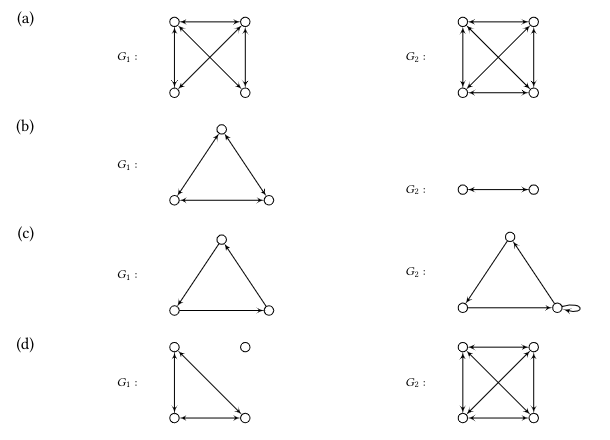
\includegraphics[width=.5\linewidth]{Assets/Logik-uebung6.png}
    \end{center}
    \begin{solution}

        a) $E_a=\exists x\exists y(\lnot x=y\wedge \lnot E(x,y))$ also $G_1\Vdash E_a$ und $G_2\not\Vdash E_a$

        b) $E_b=\exists x\exists y\exists z(x\not= y\wedge x\not= z \wedge y\not= z)$

        c) $E_c=\forall x(\lnot E(x,x))$

        d) $E_d=$
    \end{solution}

    \question Sei $\Gamma$ die Signatur bestehend aus einem zwei-stelligen Relationssymbol $\in$. Für eine Menge von Mengen $M$ definieren wir die Struktur $S$ mit $U_S=M$ und $\in^S=\in$. Geben Sie für jede der folgenden Aussagen eine Formel an, die diese beschreibt.
    \begin{parts}
        \part Es gibt eine Menge, die keine Menge enthält.
        \begin{solution}
            $\exists M: \forall x: \lnot(x\in M)$
        \end{solution}

        \part Für alle Mengen $A$ , $B$ gibt es eine Menge, die genau $A$ und $B$ enthält.
        \begin{solution}
            $\forall A,B:\exists C:\forall D: (D\in C\Leftrightarrow ((D=A)\vee(D=B)))$
        \end{solution}

        \part Für jede Menge $A$ gibt es eine Menge $B$, die genau die Elemente der Elemente der Menge $A$ enthält.
        \begin{solution}
            $\forall A:\exists B:\forall C:(C\in B \Leftrightarrow \exists D:(D\in A\wedge C\in D))$
        \end{solution}
    \end{parts}

    \question Sei $\Gamma$ die Signatur bestehend aus einem zwei-stelligen Relationssymbol $E$. Für einen (gerichteten) Graphen $G=(V,E)$ definieren wir dann die Struktur $G$ mit $V=U_G$ und $E=E^G$. Welche der folgenden Aussagen sind sind wahr? Begründen Sie Ihre Aussage!
    \begin{parts}
        \part $\{\exists x\exists y\exists z:(E(x,y)\wedge E(y,z)\wedge E(z,x))\}$ ist erfüllbar.
        \begin{solution}
            wahr: Steht ein erstes Element zu einem zweiten Element und dieses wiederum zu einem dritten Element in Relation, so steht auch das erste Element zum dritten Element in Relation. Z.B. folgt aus $a < b$ und $b<c$ stets $a<c$.
        \end{solution}

        \part $\{\exists x\forall y:E(x,y)\}$ ist erfüllbar, aber nicht allgemeingültig.
        \begin{solution}
            wahr. Es existiert ein Element, was in Relation zu allen anderen Elementen des Graphen steht, z.B. die Wurzel des Graphen.
        \end{solution}

        \part $\{\forall x\forall y:(E(x,y)\rightarrow\lnot E(y,x))\}\Vdash\forall x\forall y:(E(x,y)\wedge E(y,x)\rightarrow x=y)$
        \begin{solution}
            wahr: Es gibt keine zwei verschiedenen Elemente, die in beiden Richtungen in Relation stehen, z.B. folgt aus $a\leq b$ und $b\leq a$ stets $a=b$
        \end{solution}

        \part $\{\forall x\forall y:(E(x,y)\vee E(y,x))\}\Vdash\exists x\exists y:(E(x,y)\wedge\lnot x=y)$
        \begin{solution}
            wahr: Je zwei verschiedene Elemente stehen stets auf genau eine Weise in Relation, z.B. wenn stets entweder $a<b$ oder $b<a$ gilt.
        \end{solution}
    \end{parts}

    \question Vervollständigen Sie die unten aufgeführte Deduktion, indem Sie die verwendeten Regeln angeben und gege-benenfalls temporäre Hypothesen kenntlich machen. Welche syntaktische Folgerung wird durch die Deduktiongezeigt?
    \begin{solution}
        \begin{prooftree}
            \AxiomC{$\exists x\forall y: E(x,y)$}
            \AxiomC{$\forall y:E(x,y)$}
            \RightLabel{\scriptsize ($\forall$-E)}
            \UnaryInfC{$E(x,y)$}
            \RightLabel{\scriptsize ($\exists$-I)}
            \UnaryInfC{$\exists x:E(x,y)$}
            \RightLabel{\scriptsize ($\exists$-E)}
            \BinaryInfC{$\exists x: E(x,y)$}
            \RightLabel{\scriptsize ($\forall$-I)}
            \UnaryInfC{$\forall y\exists x: E(x,y)$}
            \RightLabel{\scriptsize ($\rightarrow$-I)}
            \UnaryInfC{$\exists x\forall y: E(x,y)\rightarrow \forall y\exists x: E(x,y)$}
        \end{prooftree}

        Folgerung: die Reihenfolge von $\exists$ und $\forall$ ist innerhalb der selben Stufe irrelevant und kann vertauscht werden: $\exists x\forall y...\rightarrow \forall y\exists x...$
    \end{solution}

    \question Sei $\sum$ eine Signatur mit dem zweistelligen Funktionssymbol $f$. Zeigen Sie durch Angabe einer geeigneten Deduktion, dass für beliebige $\sum$-Terme $s_1,s_2,t_1,t_2$ gilt: $\{s_1=t_1,s_2=t_2\}\vdash f(s_1,s_2)=f(t_1,t_2)$.
    \begin{solution}

        \begin{prooftree}
            \AxiomC{$f(s_1,s_2)$}
            \AxiomC{$[s_1=t_1]^1$}
            \RightLabel{\scriptsize (GfG$^1$)}
            \BinaryInfC{$f(t_1,s_2)$}
            \AxiomC{$[s_2=t_2]^2$}
            \RightLabel{\scriptsize (GfG$^2$)}
            \BinaryInfC{$f(t_1,t_2)$}
        \end{prooftree}
    \end{solution}

    \question Geben Sie für die folgenden (inkorrekten) Ableitungen je einen fehlerhaften Ableitungsschritt an. Begründen Sie!\\
    \begin{parts}
        \part \begin{prooftree}
            \AxiomC{$\exists x(x=a)$}
            \AxiomC{$[x=a]^1$}
            \RightLabel{\scriptsize ($\forall$-I)}
            \UnaryInfC{$\forall x(x=a)$}
            \RightLabel{\scriptsize ($\exists$-E$^1$)}
            \BinaryInfC{$\forall x(x=a)$}
        \end{prooftree}
        \begin{solution}
            Der Schritt $\forall$-I ist fehlerhaft, da x frei in $x=a$ vorkommt.
        \end{solution}

        \part
        \begin{prooftree}
            \AxiomC{$[\forall y(P(y,y))]^1$}
            \RightLabel{\scriptsize ($\exists$-I)}
            \UnaryInfC{$\exists x\forall y(P(x,y))$}
            \RightLabel{\scriptsize ($\rightarrow$-I$^1$)}
            \UnaryInfC{$\forall y(P(y,y))\rightarrow \exists x\forall y(P(x,y))$}
        \end{prooftree}
        \begin{solution}
            $\exists$-I ändert in der Hypothese y zu x, was nicht zulässig ist ($P(y,y)\not=P(x,y)$)
        \end{solution}

        \part
        \begin{prooftree}
            \AxiomC{$[\exists x(P(x))]^2$}
            \AxiomC{$[P(x)]^1$}
            \RightLabel{\scriptsize ($\exists$-E$^2$)}
            \BinaryInfC{$P(X)$}
            \RightLabel{\scriptsize ($\forall$-I)}
            \UnaryInfC{$\forall x(P(x))$}
            \RightLabel{\scriptsize ($\rightarrow$-I$^1$)}
            \UnaryInfC{$\exists x(P(x)) \rightarrow \forall x(P(x))$}
        \end{prooftree}
        \begin{solution}
            $\exists$-E fehlerhaft, da x frei in $P(x)$
        \end{solution}
    \end{parts}

    \question Wir betrachten die Formelmenge $\Gamma=\{\exists B\forall C(\lnot C\in B),\forall A\forall B\exists C(A\in C\wedge B\in C\wedge \forall D(D\in C\rightarrow C=A \vee C=B))\}$ und die Formel $\varphi=\exists C\exists B\forall A(\lnot A\in B\wedge B\in C)$ für die Signatur, die nur das zweistellige Relationssymbol $\in$ enthält. Zeigen Sie, dass $\Gamma\vdash\varphi$ gilt indem Sie eine Deduktion angeben.
    \begin{solution}

        \begin{prooftree}
            \AxiomC{$\exists B\forall C(\lnot C\in B)$}
            \AxiomC{$\forall C(\lnot C\in B)$}
            \RightLabel{\scriptsize ($\forall$-E)}
            \UnaryInfC{$\lnot A\in B$}
            \RightLabel{\scriptsize ($\forall$-I)}
            \UnaryInfC{$\forall A(\lnot A\in B)$}
            \AxiomC{$[\lnot(\forall A(\lnot A\in B))$]}
            \RightLabel{\scriptsize (iE)}
            \BinaryInfC{$\bot$}
            \RightLabel{\scriptsize ($\exists$-E)}
            \BinaryInfC{$\bot$}
            \RightLabel{\scriptsize (raa)}
            \UnaryInfC{$\forall A(\lnot A\in B)$}
            \RightLabel{\scriptsize ($\forall$-E)}
            \UnaryInfC{$\lnot A\in B$}

            \AxiomC{$\forall A\forall B\exists C(A\in B\wedge B\in C\wedge \psi)$}
            \RightLabel{\scriptsize ($\forall$-E)}
            \UnaryInfC{$\forall B\exists C(A\in B\wedge B\in C \wedge \psi)$}
            \RightLabel{\scriptsize ($\forall$-E)}
            \UnaryInfC{$\exists C(A\in C\wedge B\in C\wedge \psi$}
            \AxiomC{$[A\in C\wedge B\in C\wedge \psi]$}
            \AxiomC{$[\lnot(A\in C\wedge B\in C\wedge \psi)]$}
            \RightLabel{\scriptsize ($\wedge$-E)}
            \BinaryInfC{$\bot$}
            \RightLabel{\scriptsize ($\exists$-E)}
            \BinaryInfC{$\bot$}
            \RightLabel{\scriptsize (raa)}
            \UnaryInfC{$(A\in C \wedge B\in C)\wedge \psi$}
            \RightLabel{\scriptsize ($\wedge$-E)}
            \UnaryInfC{$A\in C \wedge B\in C$}
            \RightLabel{\scriptsize ($\wedge$-E)}
            \UnaryInfC{$B\in C$}
            \RightLabel{\scriptsize ($\wedge$-I)}

            \BinaryInfC{$\lnot A\in B\wedge B\in C$}
            \RightLabel{\scriptsize ($\forall$-I)}
            \UnaryInfC{$\forall A(\lnot A\in B\wedge B\in C)$}
            \RightLabel{\scriptsize ($\exists$-I)}
            \UnaryInfC{$\exists B\forall A(\lnot A\in B\wedge B\in C)$}
            \RightLabel{\scriptsize ($\exists$-I)}
            \UnaryInfC{$\exists C\exists B\forall A(\lnot A\in B\wedge B\in C)$}
        \end{prooftree}
    \end{solution}

    \question Geben Sie zum Beweis des Korrektheitslemmas für das natürliche Schließen in der Prädikatenlogik den Induktionsschritt für den Fall $(\exists-I)$ an.
    \begin{solution}

        I.V.: es gelte $\Gamma\vdash\varphi$, zu zeigen ist $\Gamma\Vdash\varphi$

        I.A.: mit $\varphi[x:=t]$ wird über keine Variable aus t in $\varphi$ quantifiziert.

        I.S.:
    \end{solution}

    \question In dieser Aufgabe betrachten wir Mengen von Schließregeln. Wir sagen, dass eine Menge von $R$ von Schließregeln verifizierbar ist, wenn es entscheidbar ist, ob in einer Deduktion ausschließlich Regeln aus R verwendet wurden. Beispielsweise sei $R_{nat}$ die Menge der Regeln des natürlichen Schließens. In der Vorlesung haben wir bereits gesehen, dass $R_{nat}$ verifizierbar ist.\\
    Begründen Sie jeweils kurz, dass Ihre Regelmenge die entsprechenden Eigenschaften hat. Geben Sie je eine Mengen von Schließregeln an, die\\
    \begin{parts}
        \part nicht vollständig, aber korrekt und verifizierbar ist.
        \begin{solution}

            $R_a=\{(R)\}$
            \begin{itemize}
                \item Nicht vollständig, da z.B. $\forall x(x=x)$ nicht ableitbar mit Regeln aus $R_a$
                \item Korrekt und verifizierbar, da $R_a\in R_{nat}$
            \end{itemize}
        \end{solution}

        \part vollständig, nicht korrekt, aber verifizierbar ist.
        \begin{solution}

            $R_L=\{(\bot),(F)\}$, wobei (F) die Regel $I^F$.
            \begin{itemize}
                \item Vollständig, da $\varnothing\vdash\epsilon$ f.o. $\epsilon$ durch $\frac{I}{\epsilon}$
                \item nicht Korrekt, da für jede Formel gilt $\varnothing\vdash\epsilon$ und $\varnothing\vdash\lnot\epsilon$
                \item Verifizierbar, da jede Deduktio die Form $\frac{I}{\epsilon}$ hat
            \end{itemize}
        \end{solution}

        \part vollständig und korrekt, aber nicht verifizierbar ist.
        \begin{solution}

            $R_c=\{(\Vdash)\}$ wobei $\frac{\Gamma}{\epsilon}$ gdw. $\Gamma\Vdash\epsilon$
            \begin{itemize}
                \item Vollständig und Korrekt, da $\Gamma\vdash\epsilon$ gdw $\Gamma\Vdash\epsilon$
                \item nicht verifizierbar, da die Menge der allgmeingültigen Formeln ist nicht entscheidbar.
                \item $\epsilon$ allgemeingültig $\Leftrightarrow \varnothing\Vdash\epsilon\Leftrightarrow \frac{0}{\epsilon}(I)$ ist eine Deduktion
            \end{itemize}
        \end{solution}
    \end{parts}

    \question Wir betrachten die folgenden Sachverhalte:
    \begin{itemize}
        \item Vorlesungen werden von genau einem Professor gehalten.
        \item Studierende können Vorlesungen besuchen.
        \item Studierende können den Vortragsstil eines Professors mögen.
        \item Ein Studierender besucht eine Vorlesung genau dann, wenn er den Vortragsstil des Professors mag.
        \item Jedes Objekt ist entweder ein Studierender, ein Professor oder eine Vorlesung, aber nicht Mehreres davonzugleich.
    \end{itemize}
    Bearbeiten Sie die folgenden Teilaufgaben!
    \begin{parts}
        \part Formalisieren Sie die angegebenen Sachverhalte in der Prädikatenlogik. Verwenden Sie dazu einstellige Relationssymbole $P$(rofessor), $S$(tudierender), $V$(orlesung) und zweistellige Relationssymbole $H$(ält die Vorlesung), $M$(ag den Vortragsstil), $B$(esucht die Vorlesung). Formalisieren Sie insbesondere auch zwischen welchen Objekten die Beziehungen $H$,$M$ und $B$ bestehen können.
        \begin{solution}
            \begin{itemize}
                \item $\forall x \exists y (H(x,y) \wedge \forall z(H(z,y)\rightarrow x=z))$
                \item $\forall x \forall y (H(x,y)\rightarrow P(x) \wedge V(x))$
                \item $\forall x \forall y (M(x,y)\rightarrow S(X) \wedge P(y))$
                \item $\forall x \forall y (B(x,y)\rightarrow S(x) \wedge V(y))$
                \item $\forall x \forall y (B(x,y)\leftrightarrow \exists z(M(x,z)\wedge H(z,y)))$
                \item $\forall x((S(x)\vee P(x) \vee V(x))\wedge \lnot(S(x)\wedge P(x))\wedge \lnot(S(x)\wedge V(x))\wedge \lnot(P(x)\wedge V(x)))$
            \end{itemize}
        \end{solution}

        \part Wir sagen, dass zwei Objekte $o_1$ und $o_2$ äquivalent sind (in Zeichen $o_1\sim o_2$), wenn sie gleich sind oder vom gleichen Professor gehalten werden. Weisen Sie nach, dass die resultierende Relation $\sim$ unter den gegebenen Voraussetzungen eine Kongruenz ist.
        \begin{solution}
            $\sim$ ist Kongruenz:
            \begin{itemize}
                \item Punkt 1, Äquivalenzrelation:
                      \begin{itemize}
                          \item Reflexivität: $\forall x(x\sim x)$; Sei $o_1$ ein Objekt. Dann $o_1=o_1$, also $o_1\sim o_1$
                          \item Symmetrie: $\forall x\forall y (x\sim y\rightarrow y\sim x)$; Gelte $o_1\sim o_2$ gdw
                                gdw. $o_1 = o_2$ oder $\exists p(H(p,o_1)\wedge H(p,o_2))$
                                gdw. $o_2 = o_1$ oder $\exists p(H(p,o_2)\wedge H(p,o_1))$
                                gdw. $o_2\sim o_1$
                          \item Transitivität: $\forall x\forall y\forall z(x\sim y \wedge y\sim z \rightarrow x\sim z)$; Gelte $o_1\sim o_2$ und $o_2\sim o_3$. Dann ($o_1=o_2$ oder $\exists p(H(p,o_1)\wedge H(p,o_2))$) und
                                ($o_2=o_3$ oder $\exists p'(H(p',o_2)\wedge H(p',o_3))$).
                                Falls $o_1=o_2$ oder $o_2=o_3$, dann gilt $o_1\sim o_3$.
                                Ansonsten gilt $\exists p(H(p,o_1)\wedge H(p,o_2))\wedge \exists p'(H(p',o_2)\wedge H(p',o_3))$. Da Vorlesungen von genau einem Professor gehalten werden gilt $p=p'$. Also werden $o_1$ und $o_3$ auch vom gleichen Professor gehalten. Somit $o_1\sim o_3$
                      \end{itemize}
                \item Punkt 2 gilt, da keine Funktionen in Signatur
                \item Punkt 3, Relationen:
                      \begin{itemize}
                          \item Seien $a_1,b_1,...,a_k,b_k$ so dass $a_1\sim b_1,...,a_k\sim b_k$. Gelte $S(a_1)$ und $a_1\sim b_1$. Also gilt $a_1=b_1$ oder $\exists p(H(p,a_1)\wedge H(p,b_1))$. Falls $H(p,a_1)$, dann gilt $V(a_1)$ nach (ii) doch $d_15$ widerspricht (vi). Daher muss $a_1=b_1$ gelten und somit $S(b_1)$
                          \item Für $P(a_1)$ analog
                          \item Gelte $V(a_1)$ und $a_1\sim b_1$. Falls $a_1=b_1$, dann gilt $V(b_1)$. Ansonsten $\exists p(H(p,a_1)\wedge H(p,b_1))$. Also gilt $V(b_1)$ nach (ii)
                          \item Gelte $M(a_1,a_2)$ und $a_1\sim b_1$ und $a_2\sim b_2$. Es gilt $S(a_1)$ und $P(a_1)$, also $\lnot V(a_1)$ und $\lnot V(a_2)$. Somit gilt $a_1=b_1$ und $a_2=b_2$, also $M(b_1,b_2)$
                          \item Gelte $H(a_1,a_2)$ und $a_1\sim b_1$ und $a_2\sim b_2$. Da $H(a_1,a_2)$ gilt $P(a_1)$ und $V(a_2)$. ($a_1=b_1$ oder $\exists p(H(p,a_1)\wedge H(p,b_1)))$ und $(a_2=b=2$ oder $\exists p(H(p,a_2)\wedge H(p,b_2)))$. Also gilt $a_1=b_1$. Wenn $a_2=b_2$, dann $H(b_1,b_2)$. Ansonsten $\exists p(H(p,a_2)\wedge H(p,b_2))$. Also gilt $H(b_1,b_2)$
                          \item Gelte $B(a_1,a_2)$ und $a_1\sim b_1$ und $a_2\sim b_2$. $B(a_1,a_2)$ gdw $\exists p(M(a_1,p)\wedge H(p,a_2))$ gdw $\exists p(M(b_1,p)\wedge H(p,b_2))$ gdw $B(b_1,b_2)$
                      \end{itemize}
                \item also ist $\sim$ eine Kongruenz
            \end{itemize}
        \end{solution}
    \end{parts}

    \question Sei $\sum$ eine Signatur mit einem zweistelligen Relationssymbol $E$. Im Folgenden verstehen wir $\sum$-Strukturen $G$ als unter Umständen unendliche, gerichtete Graphen $G=(U_G,E^G)$.
    \begin{parts}
        \part Geben Sie für jedes $n\in\mathbb{N}$ eine Formel $\varphi_n$ an, sodass $\psi_n$ die Klasse der Graphen axiomatisiert, in denen es einen Pfad der Länge $n$ gibt.
        \begin{solution}
            $\epsilon_n=\exists x_0 \exists x_1 ... \exists x_n(\bigwedge_{0\leq i <m } E(x_i,x_{i+1}))$
        \end{solution}

        \part Geben Sie eine unendliche Formelmenge $\phi$ an, sodass $G\Vdash\Psi$ die Klasse der Graphen axiomatisiert, in denen es beliebig lange Pfade gibt.
        \begin{solution}
            $\Phi=\{E_n| n\in\mathbb{N}\}$
        \end{solution}

        \part Zeigen Sie mithilfe des Kompaktheitssatzes der Prädikatenlogik, dass es keinen $\sum$-Satz $\psi$ gibt, der die Klasse der Graphen axiomatisiert, die nicht beliebig lange Pfade besitzen.\\
        Hinweis:Nehmen Sie an, dass es so einen Satz $\psi$ gibt und leiten Sie aus der Unerfüllbarkeit von $\phi\cup\{\psi\}$ mittels Kompaktheitssatz einen Widerspruch her.
        \begin{solution}
            Angenommen es gibt so einen Satz $\Psi$. Dann ist $\Phi\cup\{\Psi\}$ unerfüllbar. Also existiert nach Kompaktheitssatz eine endliche Teilmenge $\Phi'\subseteq \Phi\cup\{\Psi\}$, die unerfüllbar ist. Sei $m\in\mathbb{N}$ so, dass für alle $\epsilon_n\in\Phi'$ gilt $n\leq m$. Betrachte die $\sum$-Struktur $G=(U_G, E^G)$ mit $U_G=\{0,1,...,m\}, E^G=\{(i,i+1)| 0\leq i < m\}$. Dann gilt $G\Vdash \epsilon_n$ für $n\leq m$. Außerdem gilt $G\not\in\Psi$.
            Also gilt $G\Vdash \Psi' \rightarrow$ Widerspruch zur Unerfüllbarkeit. Somit kann die Annahme nicht stimmen und so ein Satz $Psi$ kann nicht existieren.
        \end{solution}
    \end{parts}

    \question Sei $f$ ein einstelliges Funktionssymbol und $R$ ein zweistelliges Relationssymbol. Weiterhin sei $$\varphi=\lnot\exists x(R(x,f(x))\wedge\forall y\exists x(R(y,x)))$$
    \begin{parts}
        \part Berechnen Sie eine Formel $\psi_1$ in Pränexform, die äquivalent ist zu $\varphi$.
        \begin{solution}
            $\psi_1 = \forall y\exists x\lnot\exists z ( R(z,f(z))\wedge R(y,x))$
        \end{solution}

        \part Berechnen Sie eine Formel $\psi_2$ in Skolemform, die erfüllbarkeitsäquivalent ist zu $\varphi$.
        \begin{solution}
            $a=\exists x; b=\lnot\exists z$

            $\psi_2 = \forall y ( R(b, f(b)) \wedge R(y, a))$
        \end{solution}
    \end{parts}

    \question Der Algorithmus zur Berechnung der Skolemform liefert für die Formel $\exists x:P(x)$ das Ergebnis $P(a)$ mit einer neuen Konstanten $a$. Zeigen Sie, dass diese beiden Formeln nicht äquivalent sind.
    \begin{solution}
        Die Variable $x$ und Konstante $a$ bilden für $P$ nur logische Äquivalenz im Fall von $x=a$, sonst nicht. Die erfüllbarkeitsäquivalenz besteht dennoch, da dies nicht von einer bestimmten Variable x abhängt.
    \end{solution}

    \question Sei $\sum$ die Signatur mit dem zweistelligen Relationssymbol $R$, der Konstante $a$ und dem zweistelligen Funktionssymbol $g$. Gegeben sei weiterhin die folgende Formel:
    $\varphi=\forall x\forall y:(R(x,g(x,y))\vee R(x,a)\wedge(\lnot R(y,x)\vee R(y,g(x,y))))$.
    Geben Sie jeweils mindestens zwei Elemente des Herbrand-Universums und der Herbrand-Expansion an.
    \begin{solution}
        $H_{\varphi} = \{a, g(a,a), R(a,a), R(g(a,a),a), ...\}$

        $E(\varphi)_1 =  (R(a,g(a,a))\vee R(a,a)\wedge(\lnot R(a,a)\vee R(a,g(a,a))))$ mit $[x/a][y/a]$

        $E(\varphi)_2 =  (R(g(a,a),g(g(a,a),a))\vee R(g(a,a),a)\wedge(\lnot R(a,g(a,a))\vee R(a,g(g(a,a),a))))$ mit $[x/g(a,a)][y/a]$
    \end{solution}

    \question Sei $\sum$ die Signatur mit dem zweistelligen Relationssymbol $R$ und den Konstanten $a$ und $b$. Betrachten Sie die folgende Formel $\varphi=\forall x\forall y:(R(a,b)\wedge(R(x,x)\rightarrow R(a,y))\wedge\lnot R(y,a))$.
    \begin{parts}
        \part Berechnen Sie die Herbrand-Expansion $E(\varphi)$.
        \begin{solution}

            $H_{\varphi} = \{a,b, R(a,b) ,...\}$

            $E(\varphi) = \{R(a,b)\wedge(R(x,x)\rightarrow R(a,y))\wedge\lnot R(y,a) | x,y\in H_{\varphi}\}$
        \end{solution}

        \part Überprüfen Sie, ob $E(\varphi)$ aussagenlogisch erfüllbar ist.
        \begin{solution}

            mit $x=a,y=a: R(a,b)\wedge(R(a,a)\rightarrow R(a,a))\wedge\lnot R(a,a)$ Nicht erfüllbar $R\wedge\lnot R$

            mit $x=a,y=b: R(a,b)\wedge(R(a,a)\rightarrow R(a,b))\wedge\lnot R(b,a)$ erfüllbar

            mit $x=b,y=a: R(a,b)\wedge(R(b,b)\rightarrow R(a,a))\wedge\lnot R(a,a)$ Nicht erfüllbar $R\wedge\lnot R$

            mit $x=b,y=b: R(a,b)\wedge(R(b,b)\rightarrow R(a,b))\wedge\lnot R(b,a)$ erfullbar

            $\rightarrow$ aussagenlogisch nicht erfüllbar
        \end{solution}
    \end{parts}

    \question Sei $\sum$ die Signatur mit dem einstelligen Relationssymbol $P$, der Konstante $a$ und den einstelligen Funktionssymbolen $f$ und $g$. Betrachten Sie die Formel $\varphi=\forall x:(P(a)\wedge(P(x)\rightarrow P(f(x)))\wedge\lnot P(g(x)))$. Weiterhin sei $A$ eine Struktur mit
    \begin{itemize}
        \item $U_A=\mathbb{Q}$,
        \item $P^A=\mathbb{N}\backslash\{0\}$,
        \item $a^A=1$,
        \item $f^A(n)=n+1$ für alle $n\in\mathbb{Q}$ und
        \item $g^A(n)=0$ für alle $n\in\mathbb{Q}$.
    \end{itemize}
    Dann kann leicht $A\Vdash\varphi$ gezeigt werden. Konstruieren Sie aus $A$ eine Herbrand-Struktur $B$, welche ebenfalls Modell für $\varphi$ ist.
    \begin{solution}

        $H_{\varphi} = \{a, f(a), g(a), ... \}$

    \end{solution}

\end{questions}
\end{document}